\titre{}
\theme{limites}
\auteur{Nathan Scheinmann}
\niveau{3M}
\source{sesamath3e}
\type{serie}
\piments{2}
\pts{}
\annee{2425}

\contenu{
\tcblower
\begin{minipage}[t]{0.4\textwidth}{
\vspace{0pt}
\noindent Déterminer, si possible :
\begin{tasks}(2)
\task \(\displaystyle\lim_{x\to 1}f(x)\)
\task \(\displaystyle\lim_{x\to -3^-}f(x)\)
\task \(\displaystyle\lim_{x\to -3^+}f(x)\)
\task \(f(-3)\)
\task \(\displaystyle\lim_{x\to 3^+}f(x)\)
\task \(\displaystyle\lim_{x\to 3^-}f(x)\)
\task \(\displaystyle\lim_{x\to 3}f(x)\)
\task \(f(3)\)
\task \(\displaystyle\lim_{x\to -1}f(x)\)
\task \(\displaystyle\lim_{x\to 4}f(x)\)
\task \(\displaystyle\lim_{x\to 2^+}f(x)\)
\task \(\displaystyle\lim_{x\to 2}f(x)\)
\end{tasks}
}
\end{minipage}
\begin{minipage}[t]{0.6\textwidth}{
\vspace{0pt}
\begin{center}
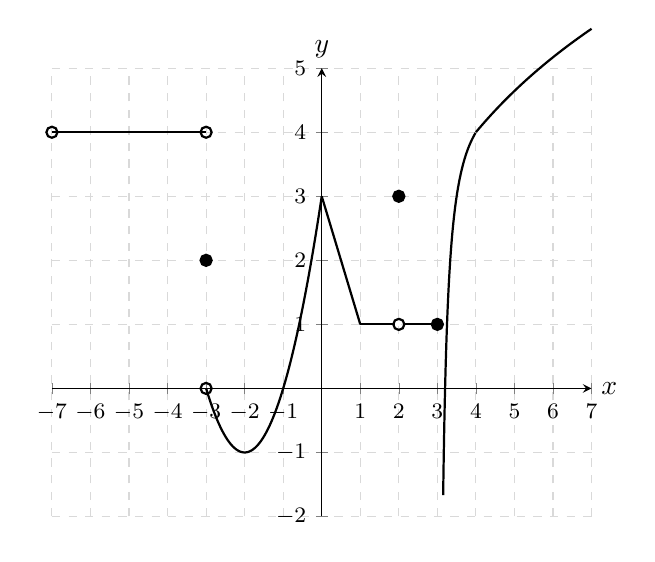
\begin{tikzpicture}
  \begin{axis}[
    axis lines=middle,
    xlabel={$x$}, ylabel={$y$},
    xlabel style={at=(current axis.right of origin), anchor=west},
    ylabel style={at=(current axis.above origin), anchor=south},
    xmin=-7, xmax=7,
    ymin=-2, ymax=5,
    xtick={-7,...,7},
    ytick={-2,...,5},
    xticklabel style={font=\footnotesize},
    % only y‐ticks (if you ever want it):
    yticklabel style={font=\footnotesize},
    %xtick=\empty, ytick=\empty,
    grid=both,
    grid style={dashed,gray!30},
    clip=false,
  ]
    % 1) f(x)=4 on (-7,-3)
    \addplot[domain=-7:-3, thick] {4};
    \addplot[only marks, mark=o, thick] coordinates {(-7,4) (-3,4)};
    %    f(-3)=2
    \addplot[only marks, mark=*, thick] coordinates {(-3,2)};
    % 2) f(x)=x^2+4x+3 on (-3,0)
    \addplot[domain=-3:0, samples=100, thick] {x^2+4*x+3};
    \addplot[only marks, mark=o, thick] coordinates {(-3,0)};
    % 3) f(x)=-2x+3 on (0,1)
    \addplot[domain=0:1, thick] {-2*x+3};
    % 4) f(x)=1 on (1,3), open at x=2 and x=3
    \addplot[domain=1:1.9, thick] {1};
    \addplot[domain=2.1:2.9, thick] {1};
    \addplot[only marks, mark=o, thick] coordinates {(2,1)};
    %    but f(2)=3
    \addplot[only marks, mark=*, thick] coordinates {(2,3) (3,1)};
    % vertical asymptote at x=3
    % 5) f(x)=1/(x-3) on (3,4)
    \addplot[domain=3.15:3.99, samples=200, thick] {1/(3-x)+5};
    % 6) f(x)=\log_{\sqrt2}(x) on [4,7]
    \addplot[domain=4:7, samples=200, thick] {ln(x)/ln(sqrt(2))};
  \end{axis}
\end{tikzpicture}
\end{center}
}
\end{minipage}
}
\correction{
	\tcblower
\begin{tasks}(6)
	\task $1$
	\task $4$
	\task $0$
	\task $2$
	\task $1$
	\task $-\infty$
	\task n'existe pas
	\task $1$
	\task $0$
	\task $4$
	\task $1$
	\task $1$
\end{tasks}
}

